\chapter{INTRODUÇÃO} \label{cap:intro}
\vspace{-2cm}

Desde o descobrimento da fissão nuclear, os estudos relativos ao tema vem se sofisticando cada vez mais. A descoberta da fissão proporcionou estudos do uso de partículas atômicas na geração de energia, o que no meio do século XX se tornou uma realidade. Em contrapartida, as estudos nucleares também possibilitaram a criação de armas de destruição em massa como a bomba atômica. Essa capacidade dual da tecnologia nuclear gerou enorme discussão no início da década de 50(?). Após a descoberta do potencial destrutivo das bombas atômicas e também do enorme potencial da energia nuclear, iniciou-se uma série de discussões para que essa nova tecnologia fosse implementada de forma pacífica e segura.
Nesse panorama, sistemas de monitoramento do uso destes sistemas são imprescindíveis de forma a assegurar que o combustível nuclear ou o refugo não estejam sendo retirados de forma não declarada da usina, como para, por exemplo, na criação de armamentos nucleares.

Uma das formas de fazer esse monitoramento é através de detectores de antineutrinos do tipo Cherenkov. A radiação de Cherenkov trata-se de uma radiação eletromagnética emitida quando uma partícula carregada eletricamente atravessa um meio a uma velocidade superior à da luz neste meio, esta radiação se dá através de fótons, geralmente no espectro do ultra-violeta, como pode ser visto na Figura \ref{fig:cherenkov}. No caso de usinas nucleares, algumas das partículas liberadas são os antineutrinos, resultantes do decaimento beta de nuclídeos gerados na fissão nuclear. Assim, uma forma de monitorar o uso do combustível é através da relação entre energia gerada e o número de antineutrinos detectados. 

\begin{figure}[H]
	\centering
		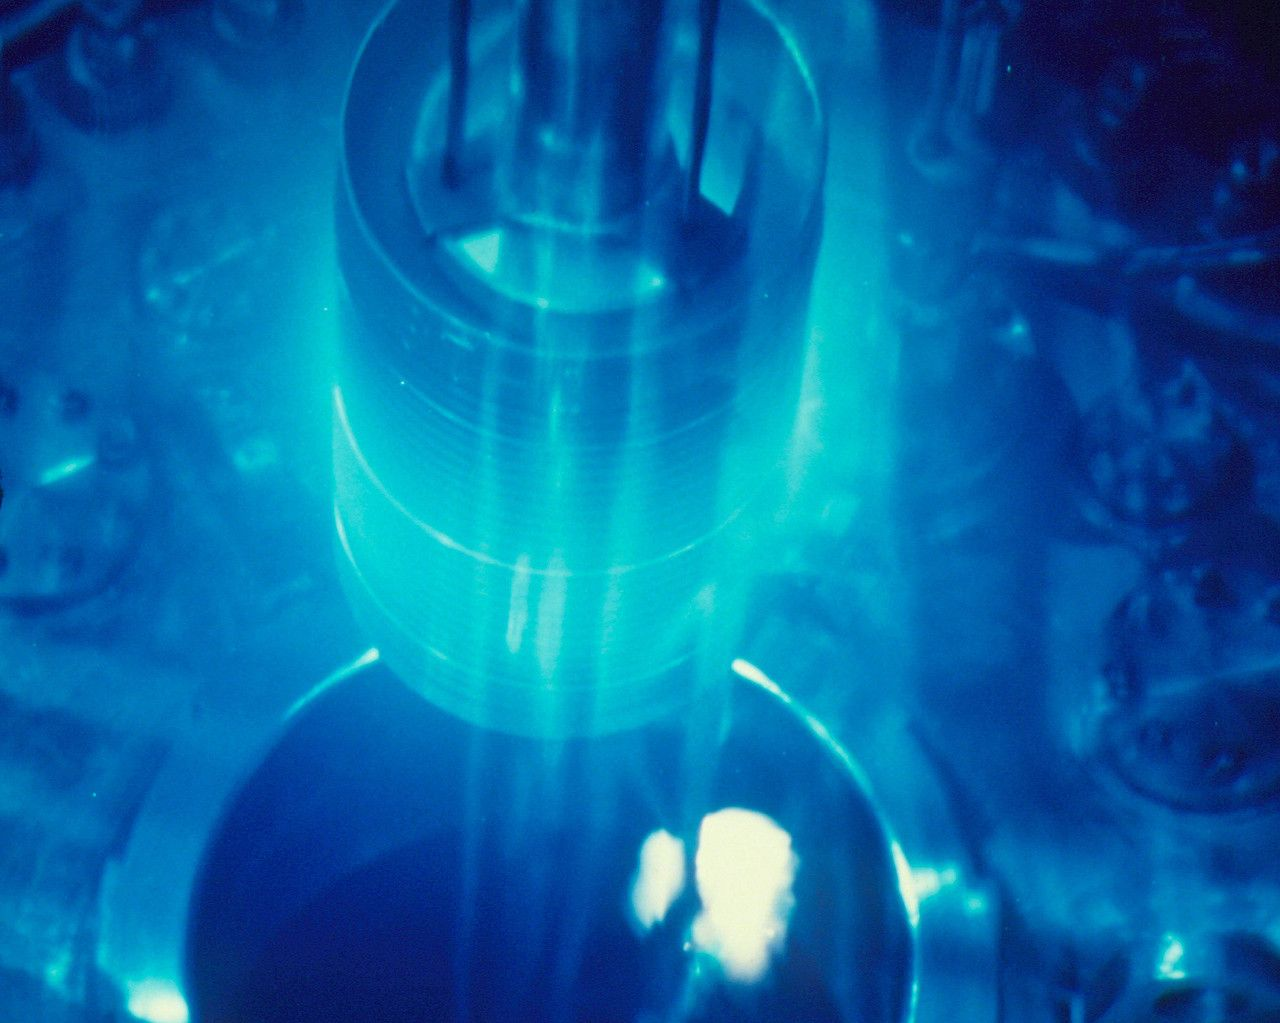
\includegraphics[width=7.7cm]{textuais/simulacao/figuras/cherenkov.jpg}
		\caption{Radiação de Cherenkov vista em um reator nuclear}
		\label{fig:cherenkov}
\end{figure}%

No Brasil, o experimento Neutrinos-Angra ($\nu$-Angra) foi criado com o intuito de medir a atividade de reatores nucleares através de um detector de neutrinos do tipo Cherenkov pela relação entre potência térmica dissipada e taxa de eventos de neutrinos registrados pelo detector. Um dos principais objetivos do experimento é inferir a quantidade de combustível nuclear utilizado no processo de geração de energia de maneira indireta, não invasiva e totalmente independente do sistema de controle e monitoramento do reator. Ferramentas deste tipo são de interesse direto de organizações internacionais, como a IAEA e a ONU, pois podem contribuir experimentalmente em pautas relacionadas à salvaguarda de material nuclear e do desarmamento nuclear. (Carr, Rachel, et al. ”Neutrino physics for Koreandiplomacy.”Science 362.6415 (2018): 649-650)

O detector proposto pela colaboração $\nu$-Angra se baseia em um detector de superfície e, por esta razão, espera-se um ruído de fundo muito grande gerado por partículas cósmicas. Devido à este ruído, simulações da interação do detector com partículas cósmicas são importantes para melhorar a análise do sistema de diferenciação entre um evento de antineutrinos ($\bar{\nu}$) advindo do consumo de material nuclear, e um evento de raios cósmicos, como múons ($\mu$). 

O escopo deste trabalho é calibrar os parâmetros da simulação aos de uma aquisição de dados reais possibilitando um trufo para eventos futuros.


%
%A salvaguarda de material nuclear 
%
%O experimento Neutrinos-Angra ($\nu$-Angra) foi criado com o intuito de medir a atividade de reatores nucleares através de um detector de neutrinos do tipo Cherenkov pela relação entre potência térmica dissipada e taxa de eventos de neutrinos registrados pelo detector. Um dos principais objetivos do experimento é inferir a quantidade de combustível nuclear utilizado no processo de geração de energia de maneira indireta, não invasiva e totalmente independente do sistema de controle e monitoramento do reator. Ferramentas deste tipo são de interesse direto de organizações internacionais, como a IAEA e a ONU, pois podem contribuir experimentalmente em pautas relacionadas à salvaguarda de material nuclear e desarmamento nuclear. (Carr, Rachel, et al. "Neutrino physics for Korean diplomacy." Science 362.6415 (2018): 649-650)
%
%O detector proposto pela colaboração $\nu$-Angra se baseia em um detector de superfície e, por esta razão, espera-se um ruído de fundo muito grande gerado por partículas cósmicas. Devido à este ruído, simulações da interação do detector com partículas cósmicas são importantes para melhorar a análise do sistema de diferenciação entre um evento de antineutrinos ($bar{\nu}$) advindo do consumo de material nuclear, e um evento de raios cósmicos, como múons ($\mu$). 
%
%O escopo deste trabalho é calibrar os parâmetros da simulação aos de uma aquisição de dados reais possibilitando um trufo para eventos futuros.

\section{Motivação} 

Para o experimento $\nu$-Angra, calibrar a simulação até que vá ao encontro dos dados reais é de essencial importância pois, com uma simulação que concorda com os dados aquistados, pode-se ajustar o sistema real com maior eficiência, além de realizar análises e prever eventos como o espectro do elétron de Michel e de um evento de antineutrino sem a interferência da saturação da eletrônica e a complexidade da resposta do detector a um evento. 

\section{Desenvolvimento}

Este trabalho tem o foco em estudar e aprimorar a simulação do experimento $\nu$-Angra realizada no \emph{Geant4}, levando em consideração a saturação dos \ac{PMTs}, da eletrônica de \emph{front-end} e da eletrônica de aquisição, e a qualidade da água do detector tendo em vista a aquisição de dados ocorrida no período de maio a julho de 2017.

\section{Mapa dos capítulos}

Dada a apresentação do tema neste capítulo, o capítulo \ref{cap:experimento} apresenta o experimento $\nu$-Angra, dissertando sobre a motivação do experimento, o reator nuclear da usina Angra 2, especificações de montagem do detector e a eletrônica de aquisição e \emph{front-end}. O capítulo \ref{cap:dadosreais} apresenta uma análise dos dados de raios cósmicos aquisitados pelo detector enquanto posicionado ao lado do reator nuclear. O capítulo \ref{cap:simulacao} apresenta a plataforma \emph{Geant4} e os parâmetros utilizados pela simulação do experimento. O capítulo \ref{cap:resultados} mostra os resultados obtidos com a simulação e compara com os dados do experimento de fato. Por fim, o capítulo \ref{cap:conclusao} conclui o trabalho e mostra previsões futuras para o ajuste da simulação do experimento $\nu$-Angra.